% Options for packages loaded elsewhere
\PassOptionsToPackage{unicode}{hyperref}
\PassOptionsToPackage{hyphens}{url}
\PassOptionsToPackage{dvipsnames,svgnames*,x11names*}{xcolor}
%
\documentclass[
  english,
  man]{apa6}
\usepackage{lmodern}
\usepackage{amssymb,amsmath}
\usepackage{ifxetex,ifluatex}
\ifnum 0\ifxetex 1\fi\ifluatex 1\fi=0 % if pdftex
  \usepackage[T1]{fontenc}
  \usepackage[utf8]{inputenc}
  \usepackage{textcomp} % provide euro and other symbols
\else % if luatex or xetex
  \usepackage{unicode-math}
  \defaultfontfeatures{Scale=MatchLowercase}
  \defaultfontfeatures[\rmfamily]{Ligatures=TeX,Scale=1}
\fi
% Use upquote if available, for straight quotes in verbatim environments
\IfFileExists{upquote.sty}{\usepackage{upquote}}{}
\IfFileExists{microtype.sty}{% use microtype if available
  \usepackage[]{microtype}
  \UseMicrotypeSet[protrusion]{basicmath} % disable protrusion for tt fonts
}{}
\makeatletter
\@ifundefined{KOMAClassName}{% if non-KOMA class
  \IfFileExists{parskip.sty}{%
    \usepackage{parskip}
  }{% else
    \setlength{\parindent}{0pt}
    \setlength{\parskip}{6pt plus 2pt minus 1pt}}
}{% if KOMA class
  \KOMAoptions{parskip=half}}
\makeatother
\usepackage{xcolor}
\IfFileExists{xurl.sty}{\usepackage{xurl}}{} % add URL line breaks if available
\IfFileExists{bookmark.sty}{\usepackage{bookmark}}{\usepackage{hyperref}}
\hypersetup{
  pdftitle={Reproducing the Analysis of Carstensen, Shavit, \& Barnes (2020)},
  pdfauthor={Yehudis Keller1},
  pdflang={en-EN},
  pdfkeywords={COVID-19, Age, Emotions, Well-Being, Pandemic},
  colorlinks=true,
  linkcolor=blue,
  filecolor=Maroon,
  citecolor=Blue,
  urlcolor=Blue,
  pdfcreator={LaTeX via pandoc}}
\urlstyle{same} % disable monospaced font for URLs
\usepackage{graphicx,grffile}
\makeatletter
\def\maxwidth{\ifdim\Gin@nat@width>\linewidth\linewidth\else\Gin@nat@width\fi}
\def\maxheight{\ifdim\Gin@nat@height>\textheight\textheight\else\Gin@nat@height\fi}
\makeatother
% Scale images if necessary, so that they will not overflow the page
% margins by default, and it is still possible to overwrite the defaults
% using explicit options in \includegraphics[width, height, ...]{}
\setkeys{Gin}{width=\maxwidth,height=\maxheight,keepaspectratio}
% Set default figure placement to htbp
\makeatletter
\def\fps@figure{htbp}
\makeatother
\setlength{\emergencystretch}{3em} % prevent overfull lines
\providecommand{\tightlist}{%
  \setlength{\itemsep}{0pt}\setlength{\parskip}{0pt}}
\setcounter{secnumdepth}{-\maxdimen} % remove section numbering
% Make \paragraph and \subparagraph free-standing
\ifx\paragraph\undefined\else
  \let\oldparagraph\paragraph
  \renewcommand{\paragraph}[1]{\oldparagraph{#1}\mbox{}}
\fi
\ifx\subparagraph\undefined\else
  \let\oldsubparagraph\subparagraph
  \renewcommand{\subparagraph}[1]{\oldsubparagraph{#1}\mbox{}}
\fi
% Manuscript styling
\usepackage{upgreek}
\captionsetup{font=singlespacing,justification=justified}

% Table formatting
\usepackage{longtable}
\usepackage{lscape}
% \usepackage[counterclockwise]{rotating}   % Landscape page setup for large tables
\usepackage{multirow}		% Table styling
\usepackage{tabularx}		% Control Column width
\usepackage[flushleft]{threeparttable}	% Allows for three part tables with a specified notes section
\usepackage{threeparttablex}            % Lets threeparttable work with longtable

% Create new environments so endfloat can handle them
% \newenvironment{ltable}
%   {\begin{landscape}\begin{center}\begin{threeparttable}}
%   {\end{threeparttable}\end{center}\end{landscape}}
\newenvironment{lltable}{\begin{landscape}\begin{center}\begin{ThreePartTable}}{\end{ThreePartTable}\end{center}\end{landscape}}

% Enables adjusting longtable caption width to table width
% Solution found at http://golatex.de/longtable-mit-caption-so-breit-wie-die-tabelle-t15767.html
\makeatletter
\newcommand\LastLTentrywidth{1em}
\newlength\longtablewidth
\setlength{\longtablewidth}{1in}
\newcommand{\getlongtablewidth}{\begingroup \ifcsname LT@\roman{LT@tables}\endcsname \global\longtablewidth=0pt \renewcommand{\LT@entry}[2]{\global\advance\longtablewidth by ##2\relax\gdef\LastLTentrywidth{##2}}\@nameuse{LT@\roman{LT@tables}} \fi \endgroup}

% \setlength{\parindent}{0.5in}
% \setlength{\parskip}{0pt plus 0pt minus 0pt}

% \usepackage{etoolbox}
\makeatletter
\patchcmd{\HyOrg@maketitle}
  {\section{\normalfont\normalsize\abstractname}}
  {\section*{\normalfont\normalsize\abstractname}}
  {}{\typeout{Failed to patch abstract.}}
\patchcmd{\HyOrg@maketitle}
  {\section{\protect\normalfont{\@title}}}
  {\section*{\protect\normalfont{\@title}}}
  {}{\typeout{Failed to patch title.}}
\makeatother
\shorttitle{Age Emotion Analysis}
\keywords{COVID-19, Age, Emotions, Well-Being, Pandemic\newline\indent Word count: X}
\DeclareDelayedFloatFlavor{ThreePartTable}{table}
\DeclareDelayedFloatFlavor{lltable}{table}
\DeclareDelayedFloatFlavor*{longtable}{table}
\makeatletter
\renewcommand{\efloat@iwrite}[1]{\immediate\expandafter\protected@write\csname efloat@post#1\endcsname{}}
\makeatother
\usepackage{csquotes}
\ifxetex
  % Load polyglossia as late as possible: uses bidi with RTL langages (e.g. Hebrew, Arabic)
  \usepackage{polyglossia}
  \setmainlanguage[]{english}
\else
  \usepackage[shorthands=off,main=english]{babel}
\fi

\title{Reproducing the Analysis of Carstensen, Shavit, \& Barnes (2020)}
\author{Yehudis Keller\textsuperscript{1}}
\date{}


\authornote{

Yehudis Keller, Department of Psychology, Brooklyn College of the City University of New York.

Correspondence concerning this article should be addressed to Yehudis Keller, 2900 Bedford Ave., Brooklyn, NY. E-mail: \href{mailto:yehudiskeller@gmail.com}{\nolinkurl{yehudiskeller@gmail.com}}

}

\affiliation{\vspace{0.5cm}\textsuperscript{1} Brooklyn College of the City University of New York}

\abstract{
This study examines whether COVID-19 has had an adverse impact on older adults' emotional well-being. Generally, age is positively correlated with emotional well-being, but during the pandemic, older adults are the most at-risk of dying frorm the virus. A sample of 945 adults ages 18-76 answered online surveys on emotional well-being. I examine pre-test data to reproduce a t-test, in order to see if my results replicate the authors' results.
}



\begin{document}
\maketitle

\hypertarget{introduction}{%
\section{Introduction}\label{introduction}}

This report reproduced the analysis of the first of the preliminary analyses as reported in Carstensen, Shavit, and Barnes (2020). The data were downloaded from \url{https://osf.io/h7uqv/} Carstensen et al. (2020) had paricipants fill out an online survey rating the frequency and intensity of certain positive and negative emotions. The results were compared to age, to see if older adults have better emotional well-being than younger adults. Previous studies show that older adults have better emotional well-being than younger adults, but since COVID-19 disproportionately affects older adults, the authors are paying attention to any changes that might occur.

\hypertarget{methods}{%
\section{Methods}\label{methods}}

\hypertarget{participants}{%
\subsection{Participants}\label{participants}}

The participants were 945 American adults from ages 18 to 76.

\hypertarget{material}{%
\subsection{Material}\label{material}}

Participants answered questionnaires about emotional well-being. There were 29 emotions in total, 16 positive and 13 negative, and they were rated for frequency and intensity. Each question was rated according to how often the emotion was experienced in the past week, using a scale from never to all or nearly all of the time (o-4).

\hypertarget{procedure}{%
\subsection{Procedure}\label{procedure}}

To score the results, the researchers took an average for each of the following: frequency of positive emotions, frequency of negative emotions, intensity of positive emotions, and intensity of negatives.

\hypertarget{results}{%
\section{Results}\label{results}}

\begin{verbatim}
## 
##  Paired t-test
## 
## data:  the_data$avg_f_pos and the_data$avg_f_neg
## t = 15.409, df = 944, p-value < 2.2e-16
## alternative hypothesis: true difference in means is not equal to 0
## 95 percent confidence interval:
##  0.4838417 0.6250760
## sample estimates:
## mean of the differences 
##               0.5544588
\end{verbatim}

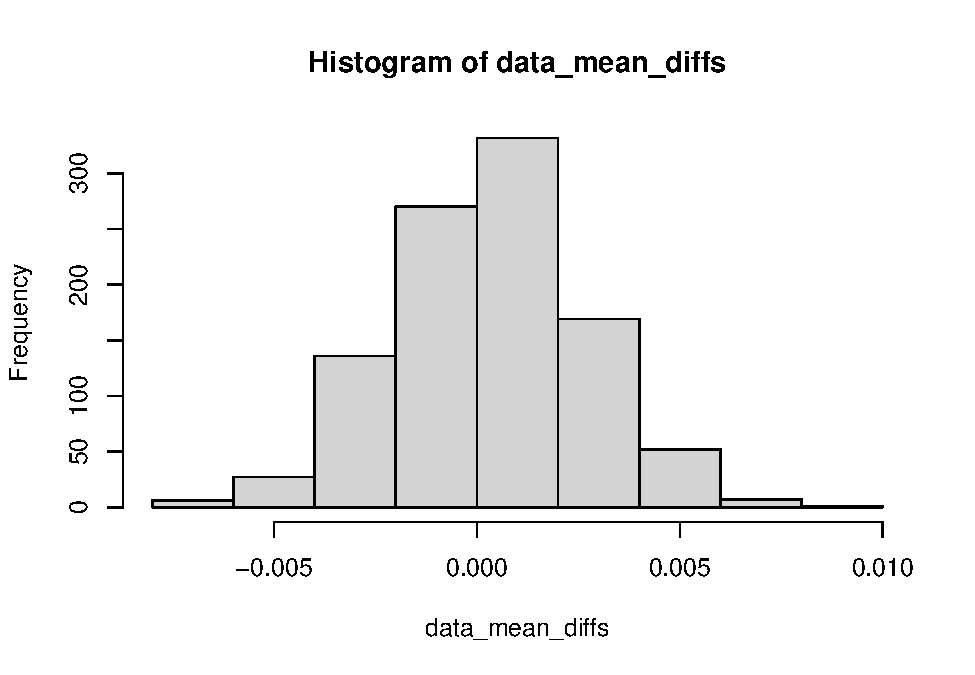
\includegraphics{APA_Rep_files/figure-latex/unnamed-chunk-1-1.pdf}

\begin{verbatim}
##         pos_mean     neg_mean
##   1: 0.001917989 0.0014109347
##   2: 0.001539202 0.0024420024
##   3: 0.002579365 0.0010582011
##   4: 0.002314815 0.0017636684
##   5: 0.002447090 0.0010582011
##  ---                         
## 941: 0.002777778 0.0007326007
## 942: 0.002040816 0.0007696008
## 943: 0.001256614 0.0025234025
## 944: 0.002976190 0.0002645503
## 945: 0.002040816 0.0017908018
\end{verbatim}

\hypertarget{reproducible-report-using-above-re-analysis}{%
\subsection{Reproducible report using above re-analysis}\label{reproducible-report-using-above-re-analysis}}

As a whole, participants reported positive emotions M = 1.97, SD = 0.56 more frequently than negative emotions M = 1.42, SD = 0.66, t(944) = 15.41, p \textless{} .2.2e-16, d = 0.53, 95\% confidence interval (CI) for the mean difference = {[}0.48, 0.63{]}. As noted above, Cronbach's alphas within valence were high for both positive and negative emotions.

\hypertarget{discussion}{%
\section{Discussion}\label{discussion}}

The re-analysis successfully reproduced the analysis reported by Carstensen et al. (2020). In the following section, I show an example of completing a simulation based power analysis for this design.

\hypertarget{simulation-based-power-analysis}{%
\subsection{Simulation-based power analysis}\label{simulation-based-power-analysis}}

The design was a paired samples design with 945 final subjects.

\begin{verbatim}
## [1] 1.559988e-87
\end{verbatim}

\begin{verbatim}
## 
##      Paired t test power calculation 
## 
##               n = 945
##               d = 0.53
##       sig.level = 0.05
##           power = 1
##     alternative = two.sided
## 
## NOTE: n is number of *pairs*
\end{verbatim}

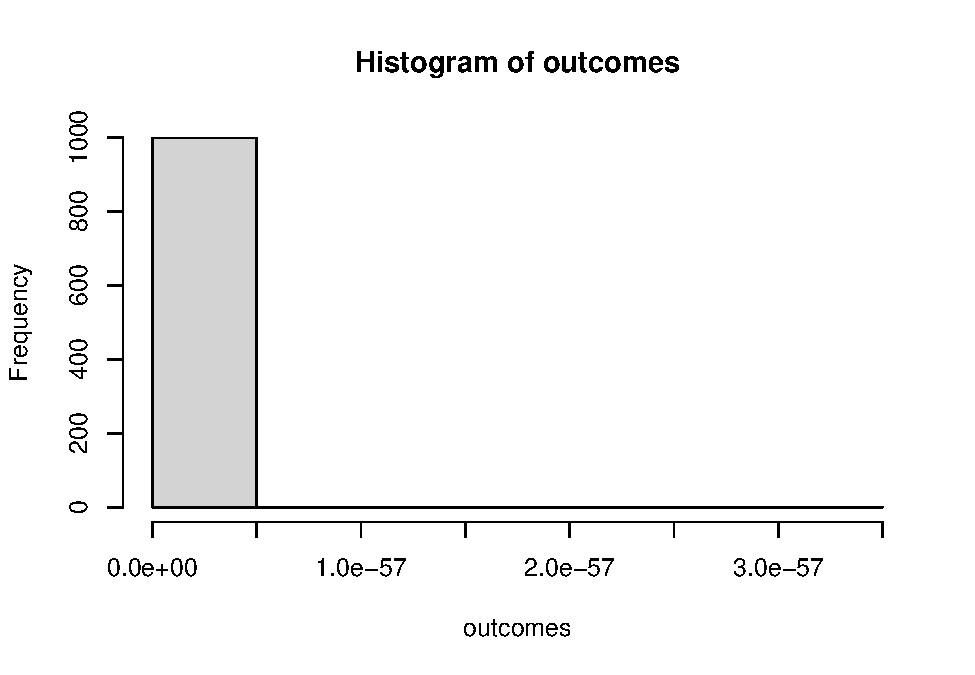
\includegraphics{APA_Rep_files/figure-latex/unnamed-chunk-2-1.pdf} 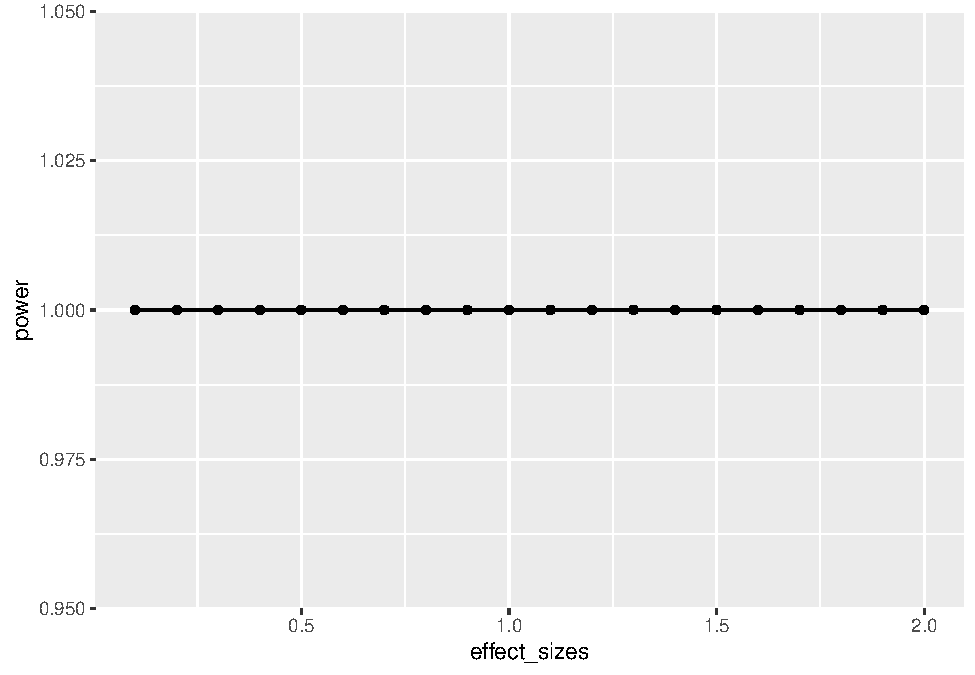
\includegraphics{APA_Rep_files/figure-latex/unnamed-chunk-2-2.pdf}
\newpage

\hypertarget{references}{%
\section{References}\label{references}}

\begingroup
\setlength{\parindent}{-0.5in}
\setlength{\leftskip}{0.5in}

\hypertarget{refs}{}
\leavevmode\hypertarget{ref-carstensen_age_2020}{}%
Carstensen, L. L., Shavit, Y. Z., \& Barnes, J. T. (2020). Age advantages in emotional experience persist even under threat from the COVID-19 pandemic. \emph{Psychological Science}, \emph{31}(11), 1374--1385. \url{https://doi.org/10.1177/0956797620967261}

\endgroup


\end{document}
